\section{DAQ and Trigger}
\subsection{Data aquisition}
\begin{frame}{The TEL-62 board}{}
	\begin{columns}
	 	\column{.45\textwidth}
			\includegraphics[width=1.15\textwidth]{tell1}
		\column{.55\textwidth}
			\begin{block}{Board with Altera Stratix III FPGAs}
				\begin{itemize}
				  \item Based on TELL-1 from LHCb
				  \item 1 Credit card PC
				  \item 4+1 Gigabit ethernet interfaces
				  \item 2 or 4 GB DDR2 memory
				  \item Up to 4 TDC daughter cards
				\end{itemize}
			\end{block}
	\end{columns}
	\begin{block}{We will have about 500 Tel-62 and similar boards at NA62}
		These boards are used for DAQ and for L0 triggering
	\end{block}
\end{frame}

\subsection{Three level online trigger}
\begin{frame}{DAQ and Trigger system}{Three levels to filter data}
	Data transmission via ordinary 10 gigabit ethernet:
	\begin{center} 
		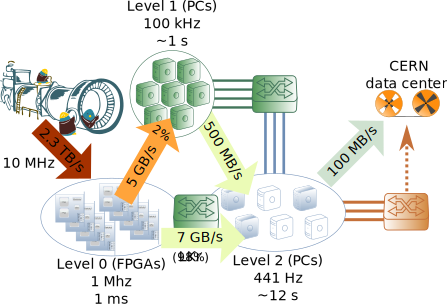
\includegraphics[width=\textwidth]{data-mitigation}
	\end{center}
\end{frame}

\begin{frame}{The Triggers}{}
	Original concept:
	\begin{block}{Level 0 (hardware)}
		$\approx$500 FPGA boards (mainly Tel-62) downstairs at the experiment
	\end{block}
	\begin{block}{Level 1 (software, on subdetector level)}
		$\approx$10 Subdetector specific PCs (8 cores with GPUs) upstairs (up to 100m
		fibre for 10G ethernet)
	\end{block}
	\begin{block}{Level 2 (software, whole detector)}
		$\approx$30 PCs (8 cores) that merge the subdetector data to one event
		(eventbuilding) and process a third trigger decision
	\end{block}
\end{frame}

\begin{frame}{The Triggers - assignments}{}
	\begin{block}{Level 0}
		Hit in the Rich, no $\gamma$ and no $\mu$
	\end{block}
	\begin{block}{Level 1}
		Every subdetector decides separately\\
		Mainly data integrity checks\\
		Ring fitting of the RICH via GPUs \\
		Track fitting for straws using GPUs planned
	\end{block}
	\begin{block}{Level 2}
		Eventbuilding (merging of all subdetector data) and reconstruction
	\end{block}
\end{frame}

\begin{frame}{First topology proposal}{}
	Original concept:
	\begin{center} 
		\includegraphics[width=0.7\textwidth]{double-star}
	\end{center}
\end{frame}